\chapter{Anforderungsanalyse}
\label{chap:anforderungsanalyse}
    Dieses Kapitel befasst sich im Allgemeinen mit der Anforderungsanalyse und -erhebung. Hierbei wird eine
    Marktanalyse präsentiert, um das Potential rundum \acl{SH} aufzuzeigen und die entstehenden oder bereits 
    bestehenden Anforderungen aufzuzeigen. Die Analyse ist 
    mit repräsentativen Statistiken, Studien und Umfragen belegt. Hauptsächlich wird im Rahmen der Anforderungserhebung 
    auf die Methodiken und Techniken eingegangen, die verwendet werden, um 
    Anforderungen zu identifizieren. Diese dienen als Grundlage für die Konzeption der Steuerzentrale. Bestandteile der 
    Anforderungserhebung sind unter anderem zentrale Prozesse des \acl{RE}, ein \textit{user-centered Design} (nutzerzentriertes Design), 
    eine \textit{Target Group Analysis} (Zielgruppenanalyse), und die Durchführung von 
    Experteninterviews. Diese Interviews sind nicht repräsentativ und dienen lediglich der weiträumigeren Informationsgewinnung. 
    \\
    Vorab wird sichergestellt, dass im Rahmen des benutzerzentrierten Designs der Softwareentwickler als Nutzer und Anwender im 
    Vordergrund steht, da dieser die Plattform betreibt, bzw. für die Erweiterung der Software als auch für die 
    Anpassungen auf die eigenen Anwendungsfälle zuständig ist.
    \\
    \linebreak
    Damit ein Eindruck entsteht, welches Marktpotential \acl{SH} Anwendungen haben und welche Anforderungen somit 
    verbunden sind, wird basierend auf bestehenden Studien, Statistiken und Umfragen eine Marktanalyse durchgeführt.

\section{Marktanalyse}
\label{sec:marktanalyse}
    Der Marktanteil rundum \acl{SH} wächst weiter an, %nimmt immer weiter zu. 
    sei es in Bezug auf die Entwicklung von neuen intelligenten Geräten, die 
    Massentauglichkeit von Geräten 
    oder die stetig wachsende Abdeckung von Anwendungsfällen und Übernahme von Aufgaben und Prozessen. Durch die Vielzahl an 
    Produktanbietern und diversen Kommunikationsmöglichkeiten ist es schwierig, eine Lösung für alle Alternativen und 
    Produktausprägungen anzubieten. Hersteller versuchen mit ihrer Produktpalette ihr eigenes Ökosystem im Bereich 
    \acl{SH} zu erstellen, um die Nutzer abhängig zu machen. Der repräsentativen Studie von Deloitte zufolge ist jedoch eine 
    Insellösung bei den Nutzern in Deutschland nicht gefragt \cite{deloitte2018}. Befragt wurden 2000 Konsumenten zwischen 
    19 und 75 Jahren. Einem geringen Anteil von 22 Prozent der 
    Befragten ist die Erweiterbarkeit des Systems mit Produkten anderer Hersteller weniger, bzw. nicht wichtig. Im Gegensatz dazu 
    empfinden 43 Prozent der Befragten die Erweiterbarkeit als wichtig und 28 Prozent als sehr wichtig \cite{deloitte2018}. 
    Demnach sollten die Hersteller eine flexiblere Einsetzbarkeit gewährleisten, damit solche Systeme den Marktdurchbruch 
    erlangen. Allerdings wird dadurch die Weiterentwicklung von Plattformen komplexer und umfangreicher, was sich wiederum als 
    Nachteil erweist. Beispielsweise sind die am weitverbreitetsten Open-Source-Plattformen, openHAB und Home Assistant, 
    vielschichtig und bilden ein großes System mit zunehmend integrierbaren Geräten ab, deren Funktionsumfang stetig steigt. 

    \subsection{Allgemeine Marktsituation und Marktprognose}
        Derzeit gibt es viele Anbieter für intelligente Produkte. Diese bieten zum einen einzelne Geräte an, die in 
        beliebige Plattformen integriert werden können und zum anderen ein eigenes Ökosystem, sofern der Anwender 
        mehrere Produkte eines Anbieters nutzen möchte. Dennoch ist in den meisten Fällen die Konfiguration der Geräte nur auf 
        den hauseigenen Plattformen möglich. Somit kann der Nutzer nicht alle Komponenten ausschließlich über eine Plattform 
        konfigurieren und steuern. 
        \\
        \linebreak
        Eine repräsentative Umfrage der \ac{SGCS} mit 1384 Teilnehmern, die im April 2022 veröffentlicht wurde, zeigt, welche 
        Anbieter in Deutschland am populärsten sind, bzw. am häufigsten von den Nutzern gekauft werden. An oberster Stelle 
        steht Philips und Samsung mit jeweils 25 Prozent und an dritter Stelle Bosch mit 23 Prozent. Weitere Anbieter können dem 
        Diagramm im Anhang (siehe \ref{appendix:brandings}) entnommen werden. Es sind jedoch nicht alle Hersteller und 
        Anbieter aufgelistet. 
        \\
        \linebreak
        Der aktuelle Markt für intelligente Produkte ist in sechs primäre Segmente aufgeteilt, die jeweils andere Anwendungsfälle 
        abdecken \cite{statista2021}:
        \begin{itemize}
            \item Kontrolle und Konnektivität: Gateways die alle Geräte jeglicher Segmente kontrollieren, intelligente Lautsprecher 
            mit dem Fokus zur Kontrolle und der digitalen Unterstützung und bspw. intelligente Steckdosen
            \item Intelligente Geräte (Smart Appliances): Kühlschrank, Waschmaschine und Geschirrspüler, Kaffeemaschine, Mikrowelle 
            und Staubsaugerroboter
            \item Sicherheit: Bewegungs-, Wasser- und Rauchmelder, Kameras und Türschlösser
            \item Heimunterhaltung (Home Entertainment): Fernseher, Entertainment-Systeme 
            \item Komfort und Licht: Intelligente LEDs, Fenster- und Tür-Sensoren etc.
            \item Energiemanagement: Thermostate und Regler, Luftqualitätsmesser etc. 
        \end{itemize}
        \pagebreak
        Die aufgelisteten Segmente werden von vielen Herstellern bedient. Der folgenden Abbildung sind die repräsentativen Schlüsselanbieter zu entnehmen:
        \begin{figure}[hbt!]
            \centering
            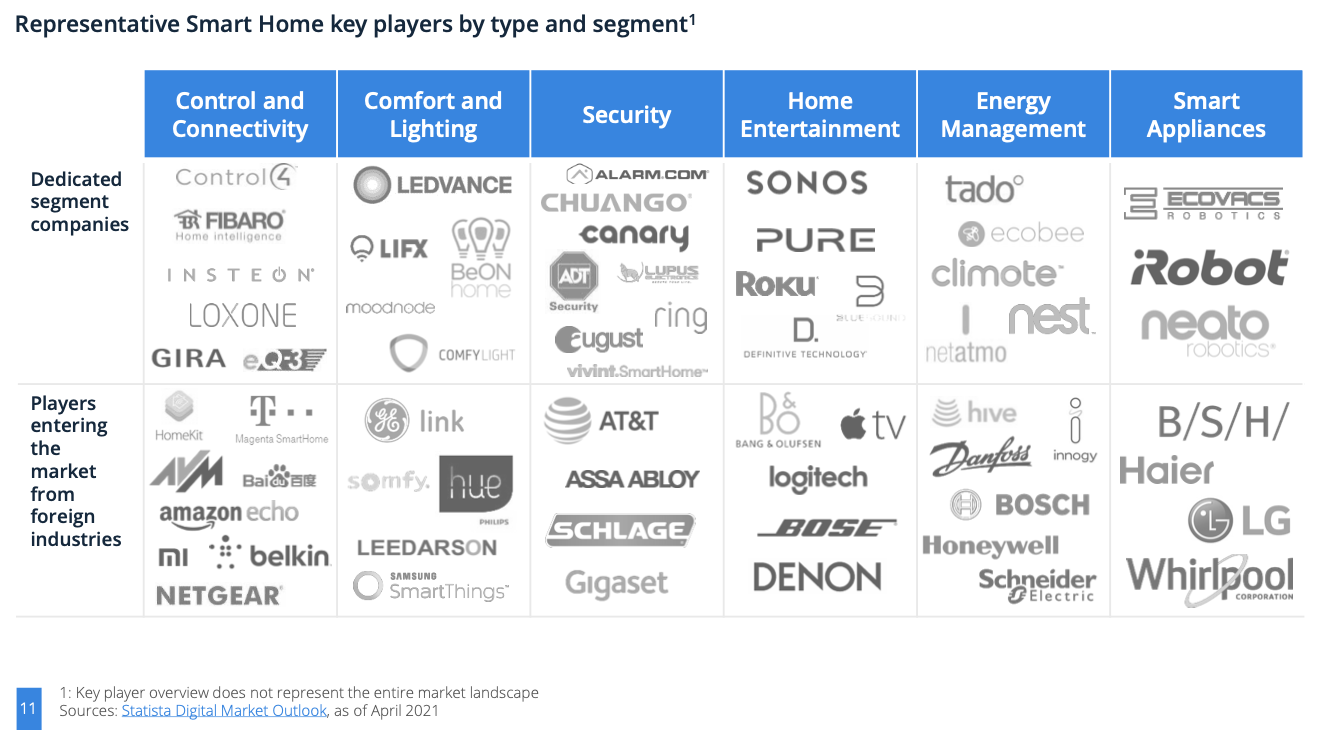
\includegraphics[width=15cm,height=10cm,keepaspectratio]{images/keyplayers.png}
            \caption{Übersicht der repräsentativen Schlüsselanbieter \cite{statista2021}} 
            \label{pic:landscape}
        \end{figure}
        \\
        Die Übersicht deckt jedoch nicht alle Anbieter ab und spezialisiert sich in diesem Fall auf die bekanntesten und die am 
        Markt etablierten. 
        \\
        \linebreak
        Laut den von Statista veröffentlichten Daten war die USA mit einem Umsatz von 28,86 Milliarden US-Dollar der größte 
        \acl{SH} Markt im Jahr 2021, wogegen Deutschland einen Umsatz von 6,59 Milliarden US-Dollar erzielte. Zu berücksichtigen sind 
        dabei jedoch die demographische Lage als auch die Bevölkerungsdichte. Diese Aufstellung steht in keinem direkten Vergleich und 
        dient lediglich zur Veranschaulichung und zur Unterscheidung der Marktanteile. Deutlich wird dabei trotzdem das ähnlich prozentual ansteigende 
        Marktwachstum. 
        \\
        \linebreak
        Der Abbildung (\ref{pic:revenue}) ist die nahezu Verdoppelung des Umsatzes bis 2026 zu entnehmen. Die Darstellung 
        (\ref{pic:globalmarket}) der einzelnen Segmente zeigt die Zunahme am Weltmarkt von 
        2021 bis 2026 um ca. 100 Prozent. Die Zeitspanne von 2019 bis 2026 stellt einen durchschnittlichen Zuwachs von 
        17,4 Prozent dar. Anhand der Prognose und des Berichts von Statista ist deutlich zu sehen, dass der \acl{SH} Markt in 
        den nächsten Jahren erheblich wachsen wird. Prognostiziert ist ein globaler Marktwert bei ca. 207,8 Milliarden 
        US-Dollar bis 2026.
        \begin{figure}[hbt!]
            \centering
            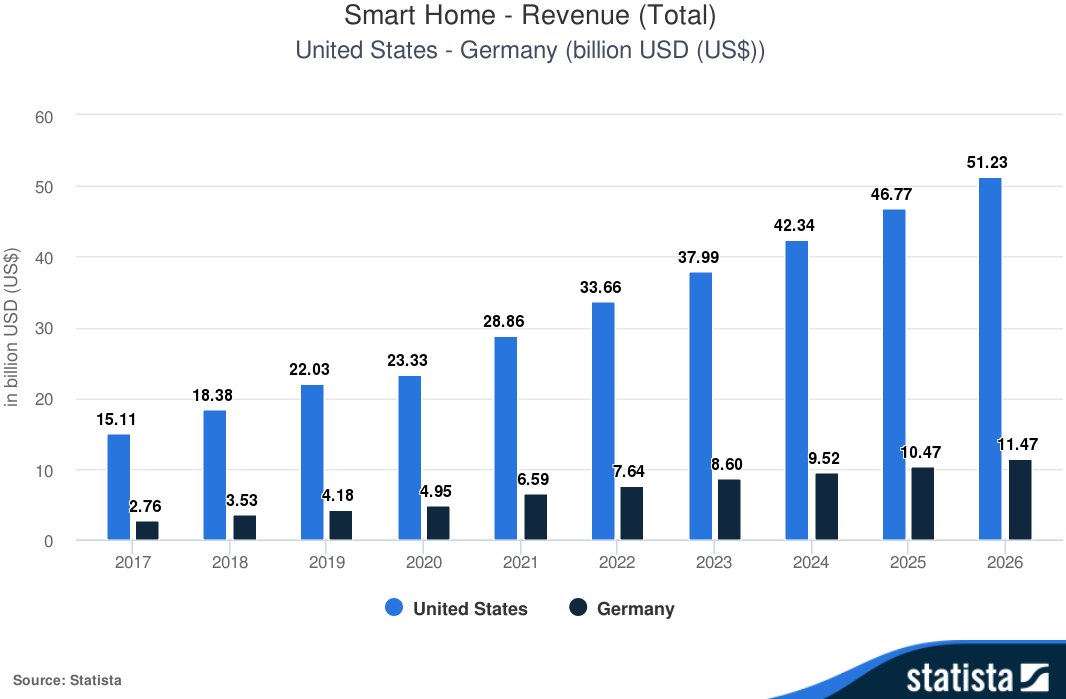
\includegraphics[width=15cm,height=9.25cm,keepaspectratio]{images/Statista-Outlook-Smart-Home---Revenue-Total-United-States---Germany-billion-USD-US.png}
            \caption{Umsatz-Prognose von Deutschland und den USA \cite{statista2021}} 
            \label{pic:revenue}
        \end{figure}
        \\
        \begin{figure}[hbt!]
            \centering
            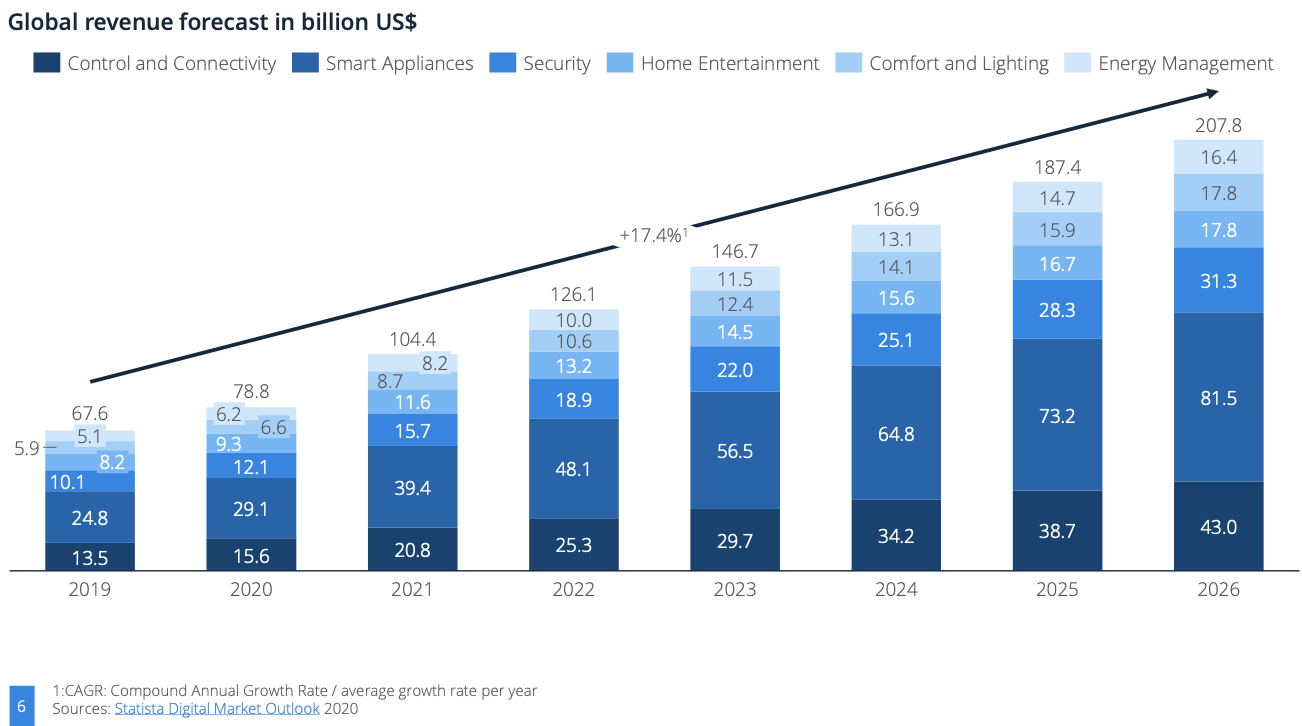
\includegraphics[width=15cm,height=10cm,keepaspectratio]{images/global_Worth_smart-home.png}
            \caption{Globaler Smart Home Marktwert \cite{statista2021}} 
            \label{pic:globalmarket}
        \end{figure}
        \pagebreak 
    \subsection*{Schlüsseltechnologien und Barrieren}
        Unter den Schlüsseltechnologien im \acl{SH} sind Komponenten zu verstehen, die den Gedanken eines intelligenten 
        Wohnraumes und Gebäudes forcieren. Dazu zählen unter anderem die Spracherkennung, die bei Sprachassistenten, 
        darunter bspw. Amazon Alexa, Apple HomePod (Siri) und dem Google Nest, eingesetzt wird, sowie \ac{AI} und \ac{KI} 
        zur Analyse, Auswertung und Optimierung von Verhaltensmustern und weiteren Analysezwecken \cite{statista2021}. 
        Zu berücksichtigen sind dabei jedoch die dafür geeigneten Anwendungsfälle und 
        die Akzeptanz der Nutzer ihre Verhaltensmuster analysieren zu lassen.
            
        \subsubsection*{Interoperabilität}
            Die Kommunikation von \acl{SH} Geräten findet meistens über drahtlose Netzwerke auf Frequenz-Bandbreiten statt, die oft nicht 
            miteinander kompatibel sind. Neben den drahtlosen Systemen gibt es auch, wie in Abschnitt (\ref{subsec:netzwerkprotokolle}) beschrieben, 
            weitere Übertragungsmethoden, darunter Strom- und Datenleitungen. Ursächlich für die Inkompatibilität der Übertragungsmethoden 
            ist die Entwicklung eines Protokolls für einen bestimmten 
            Zweck, der darauf abgestimmt ist, den Anwendungsfall abzudecken und eine Markteintrittsbarriere zu 
            schaffen, um einen Wechsel zwischen Anbietern zu erschweren \cite{statista2021}. 
            Die damit einhergehende Schwachstelle eines \acl{SH} ist, dass die Geräte mit den bereits entwickelten 
            Protokollen genutzt werden. So ist die Kommunikation über verschiedene Methoden nicht vorgesehen, was 
            eine fehlende Interoperabilität zur Folge hat. Dies würde die Kombination von Geräten erschweren oder gar verhindern, die eventuell 
            für den Anwender wünschenswert wäre. Um dies zu ermöglichen, müssten Integrationen 
            oder Plug-ins von bestehende Plattformen zur Verfügung gestellt werden oder allgemein kompatible Kommunikationsprotokolle 
            entwickelt werden, die bspw. mehrere Protokolle kombinieren können, darunter z.B. ZigBee2MQTT. 
            Voraussetzung dafür ist die Fähigkeit zur Kompatibilität und die Übereinstimmung der Technologie, auf die das Protokoll aufbaut.
            Der Anwender muss vorab selbst prüfen, welche Geräte miteinander kompatibel sind \cite{statista2021}.
            \\
            \linebreak
            Die Einführung von Bluetooth Low Energy (LE) Mesh\footnote{Bluetooth Mesh Technologie. \url{https://www.bluetooth.com} Besucht am 23.05.2022} 
            ist eine aktuelle Entwicklung, um der Herausforderung der Bewältigung der Interoperabilität einen Schritt näher zu kommen. Bei cloudbasierten 
            Sprachdiensten muss ebenso die Kompatibilität geprüft werden. 
            Neben der Datensicherheit und dem Schutz der Privatsphäre ist die fehlender Interoperabilität ein weiterer kritisch zu betrachtender Aspekt von 
            \acs{SH} Lösungen.
            \\ 
            \linebreak
            Derzeit häufig verwendete Protokolle sind unter anderem Bluetooth, \ac{WLAN} (WiFi), KNX, ZigBee, Z-Wave, 
            MQTT und weitere (siehe \ref{tab:protocolsSH}). Um Beispielsweise mit ZigBee über \acs{MQTT} kommunizieren zu 
            können, gibt es ein Framework, welches die Interoperabilität der beiden Protokolle ermöglicht. Dies ist das 
            sogenannte \textit{ZigBee2MQTT} Framework\footnote{Erschafft eine Brücke zwischen ZigBee und MQTT. \url{https://www.zigbee2mqtt.io/} Abgerufen am 23.05.2022}.
%\pagebreak
\section{Zielgruppenanalyse}
\label{sec:zielgruppenanalyse}
    Um den Adressaten dieser Arbeit näher zu definieren, erfolgt in diesem Abschnitt eine Zielgruppenanalyse. %Hierbei wird zwischen 
    %zwei Gruppen differenziert. 
    Im Rahmen dieser Tätigkeit wird die konkrete Zielgruppe identifiziert, die das Framework als Grundlage nutzt, um die individuellen 
    Anwendungsfälle in der Umgebung des Büros umzusetzen und ggf. zu erweitern. Die Verwendung des Frameworks ist nicht zwangsläufig auf die Büroumgebung beschränkt, ebenso kann 
    das Framework in privatem Gebrauch angewendet werden. Da es sich bei der Zielgruppenanalyse um einen fortlaufenden Prozess handelt, wird in dieser Arbeit die erste Iteration durchgeführt, 
    die anschließend weiter verfolgt werden kann. 
    %Im Kontext der Arbeit wird unterschieden zwischen den Benutzern, die Produkte und Softwarelösungen von Herstellern ohne 
    %sie zu verändern gebrauchen und den Anwendern, die Frameworks als Grundlage verwenden und ihren Bedürfnissen entsprechend erweitern. Der Übergang von 
    %Benutzer zu Anwender kann fließend sein. 
    
    \subsection{Ziel der Zielgruppenanalyse}
        Die Absicht einer Zielgruppenanalyse\footnote{Beschreibung der Zielgruppenanalyse und mögliche Durchführungsschritte. \url{https://www.eology.net/magazine/target-group-analysis} Abgerufen am 24.05.2022.} 
        ist die Identifizierung der Personengruppen, die als potentielle Nutzer eines Produktes 
        oder eines Marktsegmentes gelten. Diese Methodik ist ein relevantes Werkzeug in der Produktkonzeption und -entwicklung 
        als auch in der Marktforschung. Maßnahmen und Anforderungen können aus der Zielgruppenanalyse abgeleitet und 
        erarbeitet werden. 
        \\
        Ein weiteres Ziel ist das bessere Kennenlernen der Zielgruppe, um dadurch deren Bedürfnisse und Interessen 
        genauer zu identifizieren und zu betrachten. 
    
    \subsection{Zielgruppendefinition}
    \label{subsec:zielgruppendefinition}
        Zur Bestimmung einer Zielgruppe werden folgende Kriterien unter Verwendung des Prozesstemplates der \textit{Target Group Analysis} verwendet:  
        \begin{itemize}
            \item Beruf: \textit{Ist das System nur für bestimmte Berufsgruppen interessant?} - Im Kontext der Arbeit, in der sich auf das smarte Büro bezogen wird, stehen Personen mit Programmierkenntnissen im Vordergrund. 
            \item Bildung: \textit{Über welchen Bildungsstand verfügt die Zielgruppe, die das System anspricht?} - Überwiegend Personen mit Ausbildung im IT-Umfeld, sowie Akademiker im Bereich der Softwareentwicklung sind bedeutsam.
            \item Interessen: \textit{Für Personen welcher Interessengebiete ist das System relevant?} -  Personen die Innovationen vorantreiben, aktuelle und neueste Technologien und Frameworks im Bereich \acs{SH} nutzen, könnten sich für dieses Konzept begeistern.
            \item Werte: \textit{Über welche Werte verfügen die Interessenten?} - Von Bedeutung könnten die folgenden Werte sein, wie Weiterentwicklung, Ordnung, Disziplin und Selbstbestimmung, da das Framework ein selbstständiges Erarbeiten von Lösungen für Anwendungsfälle bietet. 
        \end{itemize} 
        Mithilfe der Zielgruppendefinition kann die Bestimmung und Eingrenzung der Interessenten erfolgen. Diese wird in 
        folgendem Abschnitt verwendet, um die Zielgruppe zu erläutern. Stützend dazu werden bereits erhobenen Daten durch offizielle 
        Statistiken und Umfragen genutzt.     

    \subsection{Zielgruppe} % Benutzer}
        % Smart Home - Deutschland. Zugriff: 11. Mai 2022. https://de.statista.com/outlook/dmo/smart-home/deutschland
        Die in der Marktanalyse (\ref{sec:marktanalyse}) identifizierten Segmente werden in der Abbildung 
        (\ref{pic:segments}) nochmals aufgegriffen. Hierbei wird in der repräsentativen Statistik und Prognose der 
        Statista GmbH die Nutzung des jeweiligen Segments veranschaulicht. Der Fokus dieser Prognose liegt 
        auf der verstärkten Vertretung eines Segments in einem \acl{SH} in Deutschland. Die derzeit am meisten eingesetzten 
        Segmente sind \textit{Vernetzung und Steuerung} (rot) und \textit{Komfort und Licht} 
        (gelb). Das am wenigsten genutzt Segment stellt die \textit{Gebäudesicherheit} 
        (schwarz) in der Prognose dar. Im Jahr 2021 lag die Nutzung von Geräten des Segments \textit{Vernetzung und Steuerung} 
        bei 6,6 Millionen Nutzern, dicht gefolgt von dem Segment \textit{Komfort und Licht} mit 
        6,5 Millionen Nutzern. Dagegen liegt das Segment \textit{Home Entertainment} im Jahr 2021 bei 3,8 Millionen Nutzern.
        \\
        \linebreak
        Die bis 2026 veröffentlichte Prognose sagt voraus, dass die jeweiligen Segmente stark zunehmen %werden 
        und sich jeweils vervierfachen.  
        %\pagebreak
        \begin{figure}[hbt!]
            \centering
            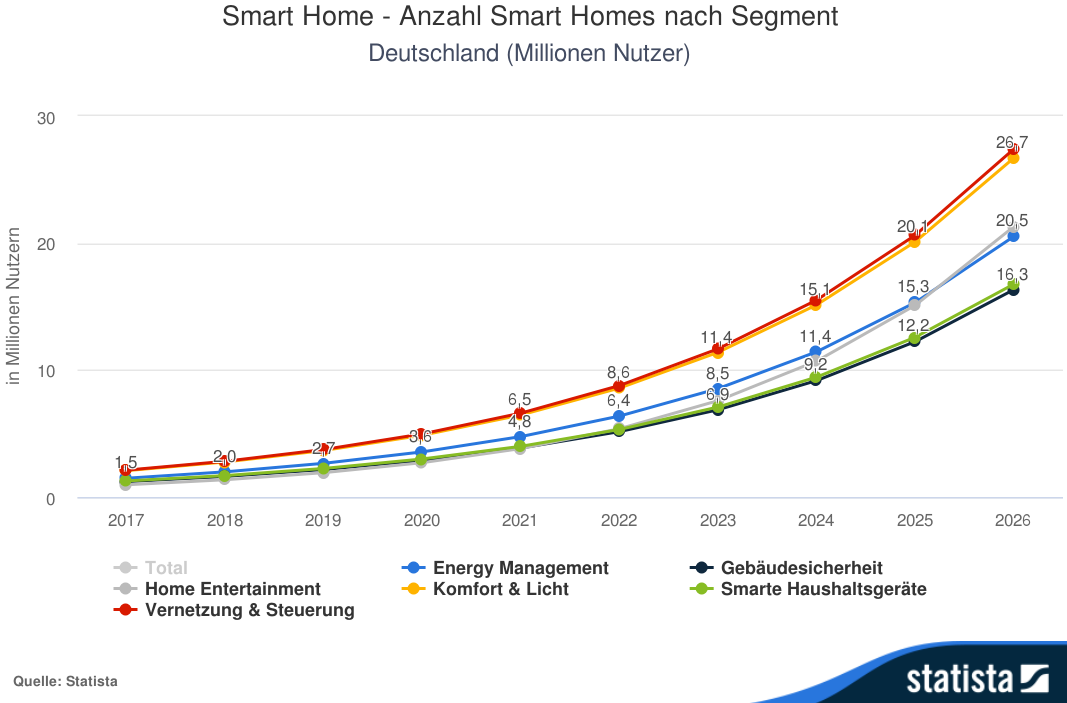
\includegraphics[width=15cm,height=10cm,keepaspectratio]{images/Statista-Outlook-Smart-Home---Anzahl-Smart-Homes-nach-Segment-Deutschland-Millionen-Nutzer.png}
            \caption{Anzahl Smart Home nach Segment \cite{statista2021}} 
            \label{pic:segments}
        \end{figure}
        \\
        Das Schaubild zeigt, dass eine bedeutende Anzahl an Personen bereits Komponenten der Segmente 
        \textit{Vernetzung und Steuerung} und \textit{Komfort und Licht} nutzen. 
        \\
        \linebreak
        %Im Hinblick auf die demographischen Statistiken ist im Jahr 2021 die Altersgruppe der 25 bis 54 Jährigen am stärksten vertreten. 
        %Der Abbildung ist weiter zu entnehmen, dass der Schwerpunkt 
        %Wobei der Abbildung (\ref{pic:ageSH}) zu entnehmen ist, dass der Schwerpunkte im Alter zwischen 45 und 54 Jahren 
        %mit 22,7 Prozent. Die Balance nach Geschlecht liegt bei einem Anteil von 45,6 Prozent weiblichen Befragten und 
        %54,4 Prozent männlichen Befragten, demnach eine geringe Ungleichheit. Die Auswertung nach Einkommen zeigt, dass 
        %35,4 Prozent der Befragten mit mittlerem Einkommen Komponenten eines \acl{SH} nutzen, dicht gefolgt von 
        %Personen mit hohem Einkommen, diese liegen bei 34,9 Prozent. 
        %\\
        %\linebreak
        %Demzufolge ist eine große Masse adressiert, die jedoch nach den Segmenten (siehe Abbildung \ref{pic:segments}) 
        %wiederum eingeschränkt werden kann.
        %\pagebreak
        %\begin{figure}[hbt!]
        %    \centering
        %    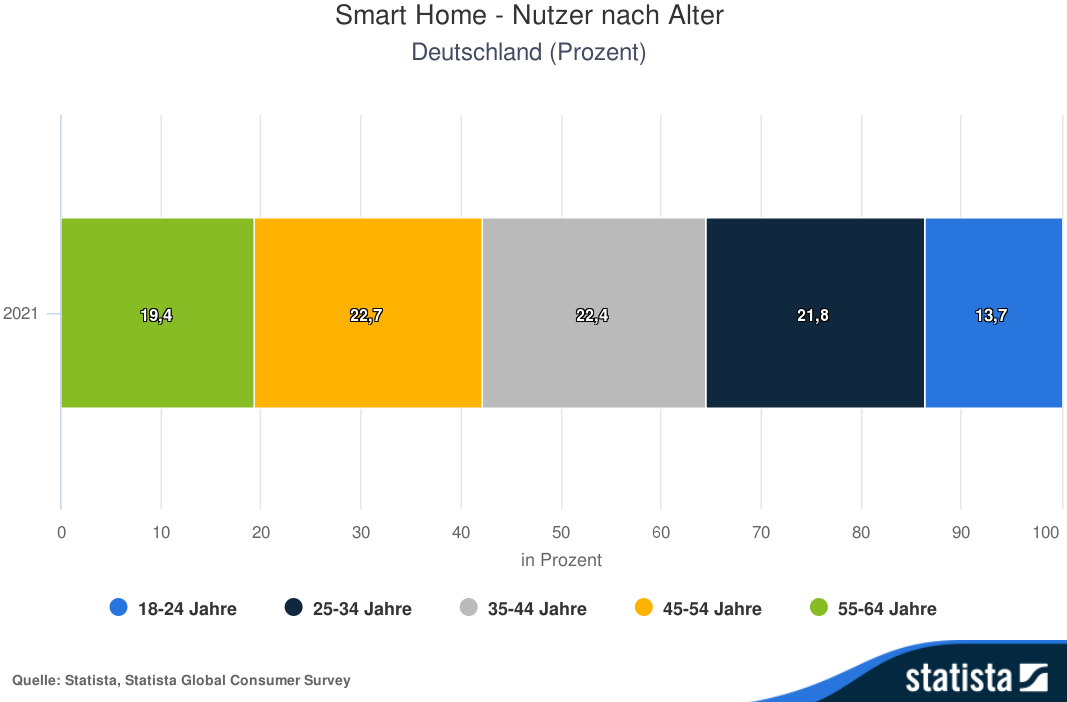
\includegraphics[width=15cm,height=10cm,keepaspectratio]{images/Statista-Outlook-Smart-Home---Nutzer-nach-Alter-Deutschland-Prozent.png}
        %    \caption{Smart Home Nutzer nach Alter \cite{statista2021}} 
        %    \label{pic:ageSH}
        %\end{figure}
        %\\
        %Die aufgeführten Statistiken und Prognosen zeigen den Markt rundum \acl{SH} auf und welches Potential für die 
        %nächsten Jahre prognostiziert wird. Im Hinblick auf die Zielgruppe lässt sich sagen, dass eine breite Masse 
        %fokussiert werden kann, die jeweils unterschiedliche Voraussetzungen und Bedürfnisse haben. Diese Analyse zeigt 
        %jedoch den gesamten Markt auf, um einen Einblick zu gewährleisten, wie stark \acl{SH} momentan in Deutschland, den 
        %Vereinigten Staaten (USA) und dem Rest der Welt vertreten ist. Um einen konkreteren Einblick 
        %zu gelangen, wird in nachfolgendem Abschnitt auf die Zielgruppe der Anwender, die in dieser Arbeit fokussiert werden, 
        %eingegangen. 
   %\subsection{Zielgruppe Anwender}
        %Die eigentliche Zielgruppe, die Softwareentwickler, die das System betreiben und für ihre Bedürfnisse anpassen.
        Der Benutzergruppe wird die Anwenderzielgruppe gegenübergestellt, diese können jedoch ebenso Benutzer der Anwendung 
        werden. Im Umkehrschluss ist ein gewisses Maß an \acs{IT}-Affinität vorausgesetzt, sodass Benutzer nicht gleich 
        Anwender sein können. Es wird eine grundlegende Kenntnis der Programmierung erfordert, im Rahmen dieser Arbeit 
        der Umgang mit der Programmiersprache Java. Einer Umfrage der Developer Nation\footnote{Umfragen, Statistiken und Berichte rundum Softwareentwickler\url{https://www.developernation.net/developer-reports/dn21} Abgerufen am 27.05.2022} 
        zufolge, benutzen von ca. 12.5 Tausend Befragten im Jahr 2021 35.8 Prozent die Programmiersprache Java. Somit kann 
        ein Rückschluss erfolgen, dass Java eine der am häufigsten verwendete Programmiersprache ist.
        \\
        \linebreak
        Im Fokus der Arbeit steht der Softwareentwickler als Anwender, welcher das System betreibt und auf die 
        individuellen Bedürfnisse anpasst. 
        \\
        Laut des Berichts der Developer Nation\footnote{Umfragen, Statistiken und Berichte rundum Softwareentwickler\url{https://www.developernation.net/developer-reports/dn21} Abgerufen am 27.05.2022}
        des dritten Quartals 2021 gibt es zu diesem Zeitpunkt 26.8 Millionen Softwareentwickler weltweit. Davon sind dem 
        Bericht von Daxx\footnote{Zusammenfassung mehrerer Berichte. \url{https://www.daxx.com/de/blog/entwicklungstrends/anzahl-an-softwareentwicklern-deutschland-weltweit-usa} Abgerufen am 27.05.2022}
        zufolge 0.9 Millionen in Deutschland angesiedelt. 
        \\
        \linebreak
        Eine vergleichbare Anwendergruppe ist die der Softwarelösung openHAB. Diese ist weltweit bekannt und zählt unter die 
        beliebtesten und am meist genutzt open source Lösungen. Anhand den eigenen Statistiken kann die Community\footnote{Website Statistik der openHAB Community. \url{https://community.openhab.org/about} Abgerufen am 27.05.2022} 
        der openHAB Foundation ca. 42 Tausend Benutzer und Anwender vorweisen. Dem GitHub Repository der \textit{openhab-core} 
        Software sind 73 Mitwirkende zugeschrieben, die dazu beitragen die Software weiterzuentwickeln, bzw. zu verbessern und zu 
        stabilisieren.
    \\
    \linebreak 
    Damit die adressierte Zielgruppe etwas greifbarer wird und die Anwendungsschritte der \textit{target group analysis} und 
    dem \textit{user-centered design} eingehalten werden, sind Persona\footnote{Eine repräsentative Vorstellung einer Person zu bestimmtem Kontext. \url{https://www.romanpichler.com/the-persona-template/} Abgerufen am 28.05.2022} 
    entwickelt worden. Diese geben die Anwenderzielgruppe wieder und geben einen Eindruck über die Personen, die sich mit dem 
    Softwareprodukt, bzw. mit dem Konzept auseinandersetzen. Die entstandenen Persona sind dem Anhang beigefügt 
    (\ref{appendix:persona}). %\ref{}

\section{Anwendungsfälle - Use Cases}
\label{sec:usecases}
    Für die Erhebung und Ausarbeitung von Anforderungen an das zu entwickelnde Framework der Steuerzentrale und dessen 
    einfache Handhabung der formalisierten Interaktionen des Softwareentwicklers wurden Anwendungsfälle, sogenannte 
    \textit{Use Cases} definiert. Diese helfen dabei, alle Anforderungen und Kriterien zu identifizieren und für das 
    Konzept zu berücksichtigen. Im Rahmen des \acl{RE} wurden die Anwendungsfälle dokumentiert und für die Konzeption, sowie 
    für die Umsetzung des Prototyps, dem \textit{Proof of Concept (PoC)}, einbezogen. 
    %zur Ergänzung von Regeln und Erweiterung des Systems und dessen 
    %Regeldefinitionen werden Anwendungsfälle, 
    %sogenannte Use Cases, definiert, bewertet und auf ihre Funktionalität geprüft. Diese wurden im Rahmen 
    %des \acl{RE} dokumentiert. 
    Das \acs{RE} nach \cite{pohl2021basiswissen} gibt Schablonen, Vorgehensmodelle und Aufgaben 
    vor, die dabei helfen, den Kontext des Projektes zu erläutern und aus den anliegenden Sachverhalten und Anwendungsfällen 
    die Anforderungen abzuleiten. Nach der strukturierten \acs{RE} Methode \ac{TORE} \cite{tore2014} werden die 
    Aufgaben, die Systemfunktionen und die Interaktionen deutlich. Zum besseren Verständnis des Kontextes und der daraus 
    resultierenden Anforderungen werden die jeweils generierten Anwendungsfälle in den folgenden Abschnitten 
    erläutert.
    \\
    \linebreak
    %Zum besseren Verständnis wird auf diese in den folgenden Abschnitten eingegangen. 
\subsection{Check-in mit einem Service-Roboter}
\label{subsec:checkin}
    Der Anwendungsfall des Check-ins mit einem Service-Roboter skizziert das Szenario und den Kontext des Sachverhaltes, als 
    auch die Komponenten, die benötigt werden, um den Anwendungsfall mithilfe des Frameworks der Steuerzentrale abzubilden. 
    Daraus können Anforderungen abgeleitet werden, die für das Konzept eine wichtige Rolle spielen. Mithilfe der 
    Erläuterung des Use Cases kann der Prozess aus mehreren Sichtweisen betrachtet werden, die zur Erhebung weiterer 
    Anforderungen beitragen können. 
    %Anhand dessen können die Schritte des Anwenders identifiziert werden, die notwendig sind, um die Interaktionen für den 
    %Softwareentwickler zu identifizieren und so zu verallgemeinern, dass die formalisierten Interaktionen einfach zu 
    %handhaben sind. Des weiteren soll durch die Komplexität der Anwendungsfälle auch ersichtlich werden, welche fundamentalen 
    %Komponenten und Konzeptentscheidungen notwendig sind, damit über die Steuerzentrale solche Anwendungsfälle abgebildet werden 
    %können.
    \\
    \linebreak
    Die Begrüßung und der Check-in eines Mitarbeiters oder angemeldeten Gastes an der Tür des Bürogebäudes erfordert mehrere Teilnehmer. 
    Darunter zählt die jeweilige Person, die den Check-in erfährt, eine Kamera, mit der die davor stehende Person authentifiziert wird, 
    ein Service-Roboter, der die Begrüßung und den Check-in durchführt und die Steuerzentrale, die den gesamten Prozess koordiniert. 
    \\
    \linebreak
    Für den Zeitpunkt des Check-ins muss die Person an 
    der Tür bekannt sein. Hierfür findet eine Authentifizierung der Person über die Kamera an der Eingangstür statt. Der 
    Authentifizierungsvorgang wird bereits als gegeben vorausgesetzt und ist kein direkter Bestandteil der Steuerzentrale. 
    \\
    Sobald eine Person über die Kamera authentifiziert wurde, wird eine \acs{MQTT}-Nachricht über ein dafür definiertes Topic 
    an den \acs{MQTT}-Broker veröffentlicht, 
    auf das die Steuerzentrale lauscht und dessen Inhalt konsumiert. Das Konsumieren des \acs{MQTT}-Topics und die damit gesendete 
    Nachricht wird als eingehendes Ereignis verwendet, worauf die Steuerzentrale reagiert. Basierend auf dem eingehenden Event, wird der 
    weitere Prozess gestartet. Nach dem Erhalt der Nachricht wird auf Grundlage des Topics diese zugeordnet und die dafür 
    vorgesehene Regel ausgeführt. Hierfür wird der Service-Roboter über die Steuerzentrale an die Tür geschickt, an der die Begrüßung 
    stattfinden soll. Nach erfolgreicher Begrüßung wird der Check-in durchgeführt, worauf die Person einen Platz buchen kann oder bei vorab getätigter 
    Buchung diese bestätigen und sich als anwesend eintragen kann. Die grobe Skizzierung ist folgendem Anwendungsfalldiagramm zu entnehmen: 
    \begin{figure}[hbt!]
        \centering
        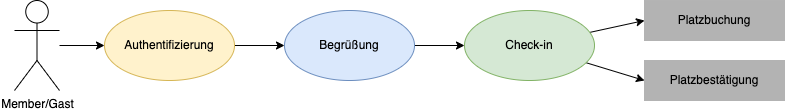
\includegraphics[width=15cm,height=15cm,keepaspectratio]{images/UC1_Diagramm_Check-in.png}
        \caption{Use Case 1 - Anwendungsfalldiagramm}
        \label{fig:uc1-check-in}
    \end{figure}
    %Der Check-in erfordert drei Teilnehmer und eine vorausgesetzte Bedingung, die bereits implementiert ist. Als Teilnehmer 
    %zählt eine Person, die den Check-in erfährt, ein Service-Roboter, der die Begrüßung und das Check-in als Anweisung 
    %durchführt und die Steuerzentrale, die den Ablauf koordiniert. Als bereits implementierter Vorgang wird die 
    %Authentifizierung der Person über eine Kamera an der Eingangstür vorausgesetzt. Diese veröffentlicht nach erfolgreicher 
    %Authentifizierung eine Nachricht an einen Nachrichten-Broker. An dieser Stelle hört die Steuerzentrale auf die 
    %veröffentlichte Nachricht und konsumiert diese. Mit dem Ereignis ist der Auslöser für die weiteren Schritte gegeben. Nach 
    %dem Erhalt der Nachricht wird diese zugeordnet und die dafür vorgesehene Regel angestoßen. Mit Beginn der Anweisung wird 
    %der Service-Roboter an die Tür geschickt, um die Person zu begrüßen.
    %\\
    %\linebreak
    %\pagebreak
    %\linebreak
    %\pagebreak
    Sobald eine Person an der Tür authentifiziert und der Begrüßungsprozess gestartet wurde, werden, während der Service-Roboter an 
    die Tür fährt, über eine Schnittstelle zur internen Büroplatzbuchungssoftware die Platzbuchungen abgefragt. 
    Sobald der Service-Roboter an der Tür angelangt ist, öffnet sich diese und die Person kann eintreten. Wenn die zu begrüßende 
    Person vor dem Service-Roboter steht, kann dieser mithilfe einer integrierten Kamera erkennen, dass eine Person gegenübersteht. 
    Zu diesem Zeitpunkt wird zur Einfachheit damit gerechnet, dass die Person, die vor dem Service-Roboter steht auch diejenige 
    ist, die an der Tür authentifiziert wurde. In zukünftiger Arbeit könnte die Person auch über die Kamera des Roboters erneut 
    authentifiziert werden, damit die Korrektheit gegeben ist. Dies ist zu diesem Anwendungsfall jedoch nicht erforderlich und 
    wird deshalb an dieser Stelle nicht weiter verfolgt.
    \\
    \linebreak
    Nachdem der Roboter die Person erkannt hat, startet die formale Begrüßung. Anschließend wird die Information der 
    vorherigen Büroplatzbuchung verwendet, um das Einchecken der Person zu starten. Wurde bei der Abfrage der Platzbuchungen ein 
    Eintrag der jeweiligen Person gefunden, so kann sich diese als anwesend einchecken und an den Arbeitsplatz gehen. Ist jedoch keine 
    Buchung gefunden worden, so kann ein freier Platz über den Roboter reserviert, bzw. gebucht werden. Die Buchung wird 
    anschließend an die Steuerzentrale zurückgegeben und über diese in das Buchungsportal eingepflegt. Nachdem dieser 
    Schritt abgearbeitet ist, endet der Anwendungsfall und der Service-Roboter wird an seine Ausgangsposition, bzw. an dessen 
    Ladestation geschickt. Somit ist das Szenario abgearbeitet und der Roboter steht für weitere Aufgaben zur Verfügung. 
    \\
    \linebreak
    Eine konkrete Aufgabenbeschreibung, sowie die User Story ist dem Anhang (sie Anhang \ref{appendix:user-story-uc1}) zu entnehmen. 
    \\
    Zur besseren Veranschaulichung des Anwendungsfalls sind die Prozesse visualisiert und folgenden Diagrammen, darunter 
    einem Aktivitätsdiagramm, einem Sequenzdiagramm und einem Ablaufdiagramm, zu entnehmen: 
    
    %im Anhang (%\ref{}%
    %SIEHE REFERENZ TBD) eine weitere Aufgabenbeschreibung, sowie die User Story als auch ein Use Case-, 
    %Sequenz- und Ablaufdiagramm zu finden.

